\documentclass[11pt]{article}

\usepackage[margin=1in]{geometry}
\usepackage{graphicx}
\usepackage{booktabs}
\usepackage{array}
\usepackage{hyperref}
\usepackage{xcolor}
\usepackage{amsmath}
\usepackage{microtype}

\hypersetup{
  colorlinks=true,
  linkcolor=blue!45!black,
  citecolor=blue!45!black,
  urlcolor=blue!45!black
}

\newcommand{\model}[1]{\textsc{#1}}

\title{Dental Vision Benchmark: A Clinician-Reviewed, Contamination-Aware Evaluation of Vision Language Models on Non-Radiographic Dental Images}

\author{
Francisco Teixeira Barbosa\\
Periospot; Foundation for Oral Rehabilitation\\
\texttt{francisco@for.org}
\and
Daniel Robles Cantero\\
Dens-IA Dental Group Research, Faculty of Health Sciences,\\
Universidad Europea Miguel de Cervantes (UEMC), Valladolid, Spain\\
\texttt{drobles@clinica.uemc.es}
}

\date{June 16, 2026}

\begin{document}

\maketitle

\begin{abstract}
Clinicians already show vision language models a diagram, an illustration, or a clinical photograph and ask ``what is this?'', but existing public dental benchmarks emphasize radiographs, closed question answering, or large-scale labeling, and few measure open-ended, caption-free reading of non-radiographic images against an explicit clinician pass/fail rubric.
We present a small, clinician-authored, contamination-aware benchmark of \emph{non-radiographic} dental image understanding: 90 openly licensed images (52 diagrams and 38 clinical photographs) across about a dozen broad categories, each paired with explicit \emph{must identify} and \emph{must avoid} rubric criteria and a reference caption.
Six contemporary vision models were evaluated through OpenRouter on June 15, 2026, with the caption stripped and no tool or web access (a leakage guard), and each free-text description was graded by two independent judges from different vendors that each see the image and the rubric.
\model{Gemini 3.1 Pro} led at 72\% (95\% Wilson interval [62, 80]), followed by \model{Claude Opus 4.8} at 63\% [53, 73] and \model{Qwen3.7 Plus} at 61\% [51, 71]; these three are statistically indistinguishable under paired McNemar tests, so the ordering is not resolved.
The robust finding is task dependence, not a resolved ranking: readable text labels strongly raise the odds of a passing description, and unlabeled clinical photographs are the hardest condition, where the weaker models fall to 20--29\%.
The two judges agreed on 82\% of descriptions (Cohen's $\kappa=0.65$), so absolute pass rates are judge-dependent.
Ground truth was reviewed by the periodontist author and independently confirmed by a second dentist (90/90 items judged clinically fair).
A transformed-control item did not reveal an obvious exact-image recognition signal, though a single control item cannot establish the absence of contamination.
The images, rubrics, per-row results, judge verdicts, and analysis code are released for reproducible, specialty-specific evaluation.
\end{abstract}

\section{Introduction}

Vision language models are now routinely shown medical images and asked to interpret them. General medical multimodal benchmarks have grown quickly, but they favor breadth and a closed question-answering format: OmniMedVQA spans 12 imaging modalities and more than 118{,}000 images, and reports that most models only slightly exceed random guessing \cite{hu2024omnimedvqa}; GMAI-MMBench is built from 284 datasets across 38 modalities, where even a leading proprietary model reached only 53.96\% \cite{chen2024gmaimmbench}. These suites measure option elimination at scale, not whether a model produces a clinically faithful free-text reading of a single image.

Dentistry is underrepresented in this literature, and the dental work that does exist is dominated by \emph{radiographs}. OralMLLM-Bench evaluates models across periapical, panoramic, and lateral cephalometric radiographs and documents a persistent gap between models and clinicians \cite{wang2026oralmllm}. Large oro-dental datasets pair intraoral images and radiographs with clinical records \cite{lv2026orodental}, and text-centric efforts such as DentalBench measure factual dentistry knowledge rather than image reading \cite{zhu2025dentalbench}. Most directly, MetaDent released a large-scale dentistry image resource (60{,}669 images with an expert-annotated subset) and benchmark suites for visual question answering, multilabel classification, and captioning, built mainly on intraoral clinical photographs with semi-structured meta-labels \cite{li2026metadent}. The closest analog to the present work evaluated six model endpoints on oral and maxillofacial anatomy using landmark identification on atlas plates, where the best endpoint reached 53.1\% and the authors concluded that no model is reliable enough to serve as a stand-alone answer key \cite{nguyen2025omf}.

Non-radiographic dental image reading, the diagrams, illustrations, and clinical photographs a clinician or student encounters daily, remains under-served: the dental benchmarks above emphasize radiographs, closed question answering, or large-scale labeling and annotation (as in MetaDent) rather than open-ended, rubric-graded reading. We therefore contribute a deliberately small, fully public, clinician-authored benchmark with three design commitments that these resources do not jointly provide: open-ended free-text grading against an explicit clinician pass/fail rubric, a leakage guard that removes the caption and any web access at input, and a transformed-control check for exact-image recognition, with per-row dual-judge auditability. We treat the model judge as an empirical quantity, reporting inter-judge agreement rather than assuming it, in line with work on LLM-as-judge reliability \cite{zheng2023judge,arora2025healthbench} and self-preference bias \cite{panickssery2024selfrecognition,wataoka2024selfpreference}.

\section{Methods}

\subsection{Benchmark dataset}

The benchmark contains 90 dental images: 52 diagrams or illustrations and 38 clinical photographs, across about a dozen broad categories (tooth and periodontal anatomy, periodontology, caries, restorative dentistry, endodontics, implants, orthodontics and occlusion, oral pathology and mucosal lesions, developmental anomalies, tooth wear, trauma, and temporomandibular or salivary structures). Radiographic interpretation is deliberately out of scope; it is a separate, harder competency and is treated as a later tier. Forty-one images carry readable text labels and 49 do not. All images are openly licensed (Wikimedia Commons or open-access sources); per-image attribution is released with the dataset.

Each image is paired with a clinician-authored rubric rather than its original web caption: a set of \emph{must identify} points that a correct reading must cover, a set of \emph{must avoid} errors, and a reference caption. A description is scored correct only if it covers all required points and commits no prohibited error. Disease severity, when applicable, is recorded but reported as a soft metric and does not gate the pass/fail score.

\subsection{Models and execution}

We evaluated six vision-capable models, the strongest of each model family available on OpenRouter on the run date (Table~\ref{tab:models}). Two strong open-weight releases of the period, GLM-5.2 and Rio 3.5, are text-only and therefore cannot enter a vision benchmark. Each image was shown to each model once at temperature 0, with a 1{,}500-token description budget. OpenRouter routed each request to an upstream provider: \model{Claude Opus 4.8}, \model{GPT-5.5}, \model{Qwen3.7 Plus}, and \model{GLM-4.6V} resolved to a single provider each (Anthropic, OpenAI, Alibaba, and Novita respectively), \model{Gemini 3.1 Pro} was served almost entirely by Google, and \model{Llama 4 Maverick} was distributed across four providers (Parasail, Google, DeepInfra, and Novita). The per-row provider is recorded in the released results and the run manifest. The run was executed on June 15, 2026; 7 of the model rows hit transient generation or judge errors and were re-run on June 16, 2026. It produced 540 description rows over the 90 primary images; a single transformed control image (run identically) adds 6 further rows that are excluded from the primary pass-rate estimates.

\begin{table}[t]
\centering
\caption{Model roster. Identifiers are the OpenRouter identifiers recorded by the harness on the run date.}
\label{tab:models}
\begin{tabular}{lll}
\toprule
Label & OpenRouter model identifier & Vendor \\
\midrule
Gemini 3.1 Pro & \texttt{google/gemini-3.1-pro-preview} & Google \\
Claude Opus 4.8 & \texttt{anthropic/claude-opus-4.8} & Anthropic \\
Qwen3.7 Plus & \texttt{qwen/qwen3.7-plus} & Alibaba \\
GPT-5.5 & \texttt{openai/gpt-5.5} & OpenAI \\
GLM-4.6V & \texttt{z-ai/glm-4.6v} & Zhipu AI \\
Llama 4 Maverick & \texttt{meta-llama/llama-4-maverick} & Meta \\
\bottomrule
\end{tabular}
\end{table}

\subsection{Leakage guard}

Each model received only the image, encoded inline as a base64 data URI, with the caption removed and with no tools or web access. Because the model cannot retrieve the original caption, a high score should reflect reading the picture rather than recalling associated text. The caption is withheld from the contestant but is given to the judges as ground truth, so this guard limits input-side recall; it does not by itself certify that a passing description was read from the pixels. The full pipeline is shown in Figure~\ref{fig:flow}.

\begin{figure}[t]
\centering
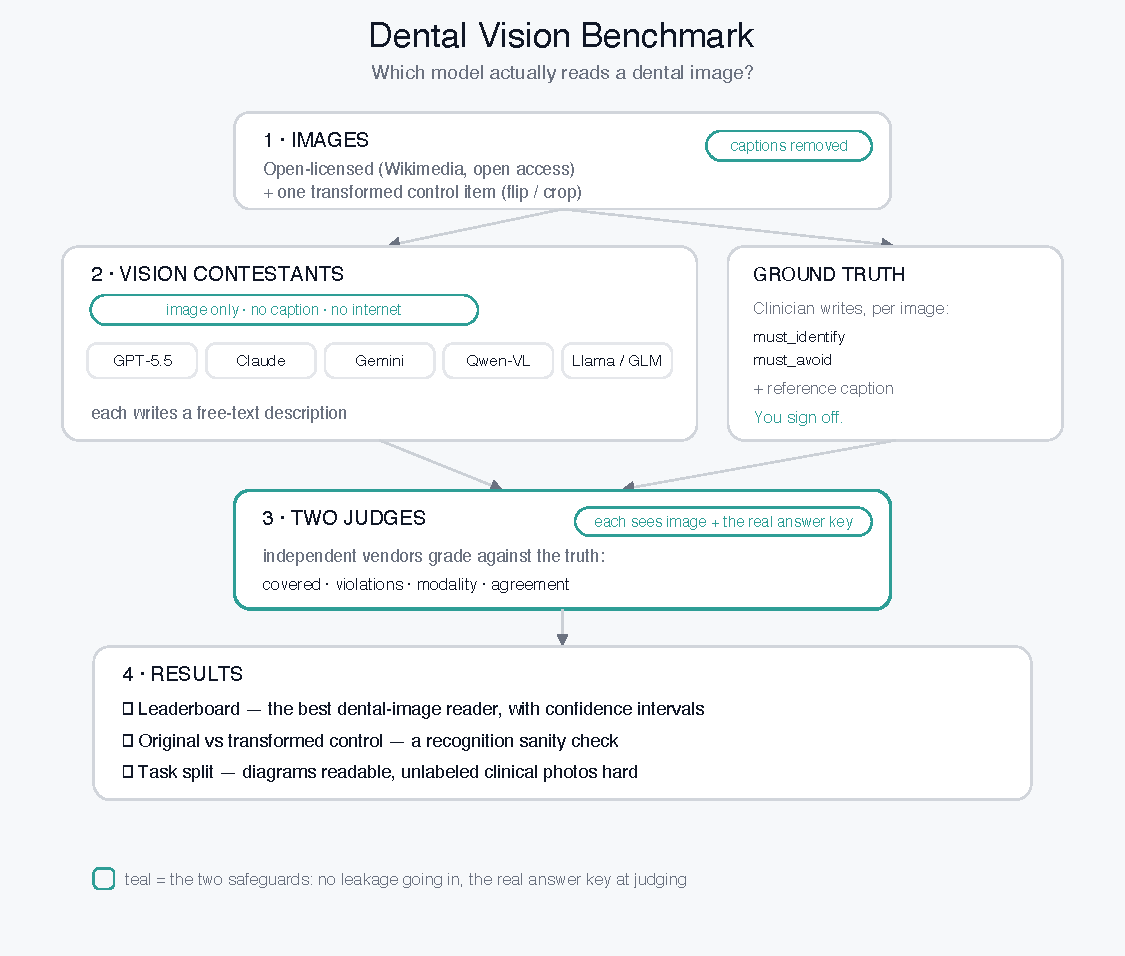
\includegraphics[width=0.86\linewidth]{figures/flow.pdf}
\caption{Benchmark pipeline. Images are shown caption-free to each vision model; two independent judges that each see the image and hold the clinician rubric grade every description; the outputs are a leaderboard with confidence intervals, a transformed-control check, and the diagram-versus-photo task split.}
\label{fig:flow}
\end{figure}

\subsection{Dual-judge rubric scoring}

Two independent judges from different vendors graded each description: a primary judge (\model{Claude Opus 4.8}) and a secondary judge (\model{GPT-5.5}). Each judge was shown the real image together with the authoritative caption and the clinician rubric, and returned a structured verdict containing the number of required points covered, the total required, the number of prohibited violations, a modality-correctness flag, and a soft severity judgment. Neither judge was shown the contestant model's identity or provider; each saw only the image, the authoritative caption, the rubric, and the description text, so the judges are blind to which model produced a description. The primary judge drives the reported leaderboard; the secondary judge quantifies judge dependence. Both judges' full verdicts are stored per row.

\subsection{Transformed control}

A transformed public control item, a flipped-and-cropped copy of one public image, is a sanity check on exact-image recognition: a model that reads the picture should score the same on the control. This is a control, not a memorization measurement.

\subsection{Outcomes and statistics}

The primary outcome is rubric pass rate per model over the 90 images. For per-model uncertainty we report 95\% Wilson score intervals. We report task splits (diagram versus clinical photograph, labeled versus unlabeled), modality-identification accuracy, a sensitivity analysis excluding 10 items pre-flagged as weak or ambiguous, and inter-judge agreement (raw verdict agreement and Cohen's $\kappa$). Because the models share the same items, model comparisons are paired by item: we additionally report McNemar exact tests with Holm correction and item-level bootstrap intervals for pairwise differences, a mixed-effects logistic model with a random intercept per image (fit as a Bayesian binomial mixed GLM via variational Bayes, so its intervals are approximate posterior credible intervals), and a rubric-burden analysis. These per-model Wilson intervals reflect a 90-image set and should not be read as population-level confidence intervals over all dental images.

\subsection{Clinician validation}

Ground truth was authored and reviewed by the periodontist author through a per-image confirm-by-default review (87 of 90 confirmed as authored; 3 corrected, comprising two rubric relaxations and one mislabeled image replaced and re-authored). A second, independent dentist (D.R.C.) then reviewed all 90 items against the released ground truth through a structured validation page and confirmed every item as clinically fair, with no rubric edits and no exclusions. The validation record is released with the repository.

\section{Results}

\subsection{Overall pass rate}

Across the 540 description rows, primary-judge pass rate was 52\%. Per-model results are shown in Table~\ref{tab:results} and Figure~\ref{fig:accuracy}. \model{Gemini 3.1 Pro} led at 72\% (65/90), followed by \model{Claude Opus 4.8} at 63\% (57/90), \model{Qwen3.7 Plus} at 61\% (55/90), \model{GPT-5.5} at 56\% (50/90), \model{GLM-4.6V} at 34\% (31/90), and \model{Llama 4 Maverick} at 28\% (25/90).

\begin{table}[t]
\centering
\caption{Primary benchmark results (primary judge). Pass rate with 95\% Wilson intervals over 90 images, and pass rate within each task split.}
\label{tab:results}
\begin{tabular}{lrrrrr}
\toprule
Model & Pass rate (95\% CI) & Diagrams & Clinical photos & Labeled & Unlabeled \\
\midrule
Gemini 3.1 Pro & 72\% [62, 80] & 71\% & 74\% & 76\% & 69\% \\
Claude Opus 4.8 & 63\% [53, 73] & 69\% & 55\% & 76\% & 53\% \\
Qwen3.7 Plus & 61\% [51, 71] & 67\% & 53\% & 71\% & 53\% \\
GPT-5.5 & 56\% [45, 65] & 63\% & 45\% & 68\% & 45\% \\
GLM-4.6V & 34\% [25, 45] & 38\% & 29\% & 41\% & 29\% \\
Llama 4 Maverick & 28\% [20, 38] & 33\% & 21\% & 27\% & 29\% \\
\bottomrule
\end{tabular}
\end{table}

\begin{figure}[t]
\centering
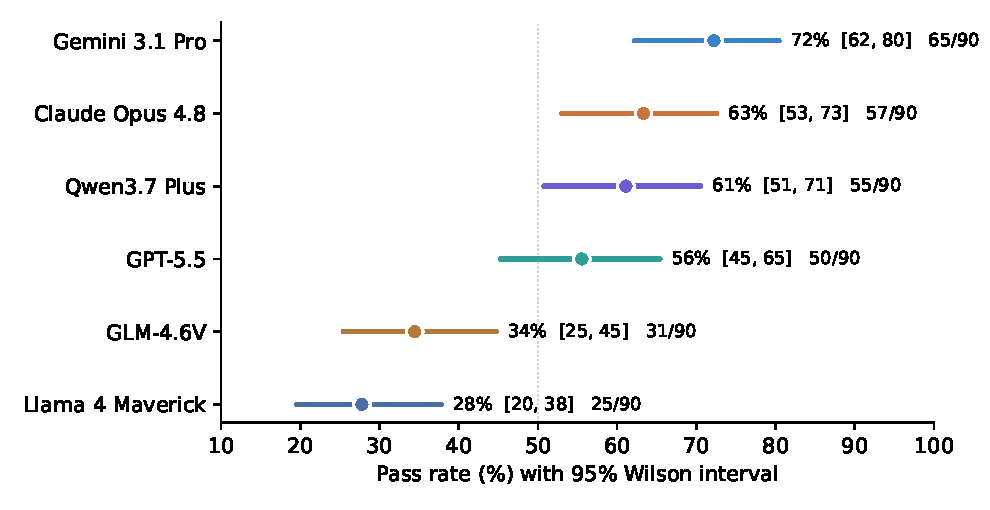
\includegraphics[width=0.86\linewidth]{figures/accuracy_by_model.pdf}
\caption{Pass rate by model with 95\% Wilson intervals over the 90 images. The top three intervals overlap; the ordering within that cluster is not statistically resolved.}
\label{fig:accuracy}
\end{figure}

The top three models form a cluster whose intervals overlap substantially, and this study should not be cited as evidence of a resolved ordering among them. The more informative separation is between this leading cluster and the lower-performing tail. Notably, \model{GPT-5.5} sits below the cluster here, even though the OpenAI family is among the strongest systems on text-based clinical question answering; strength on text need not transfer to vision. A sensitivity analysis excluding the 10 pre-flagged weak or ambiguous items (n$=$80) shifted every model upward by 3 to 5 points and left the ranking unchanged.

\subsection{The task split is the headline}

Figure~\ref{fig:split} and the right-hand columns of Table~\ref{tab:results} show the robust result. Across the field, diagrams and labeled images are read more reliably than unlabeled clinical photographs. The gap is largest for the mid and lower tier: \model{GPT-5.5} falls from 63\% on diagrams to 45\% on unlabeled images, and \model{GLM-4.6V} and \model{Llama 4 Maverick} fall to 29\% and below on unlabeled images. \model{Gemini 3.1 Pro} is the exception, reading clinical photographs (74\%) as well as diagrams (71\%). Reading an unlabeled real mouth, rather than a textbook diagram, is the hard and still unsolved part of this task. Modality identification, by contrast, was nearly saturated: every model labeled diagram versus photograph correctly about 99\% of the time, so the failures are in clinical reading, not image-type confusion.

\begin{figure}[t]
\centering
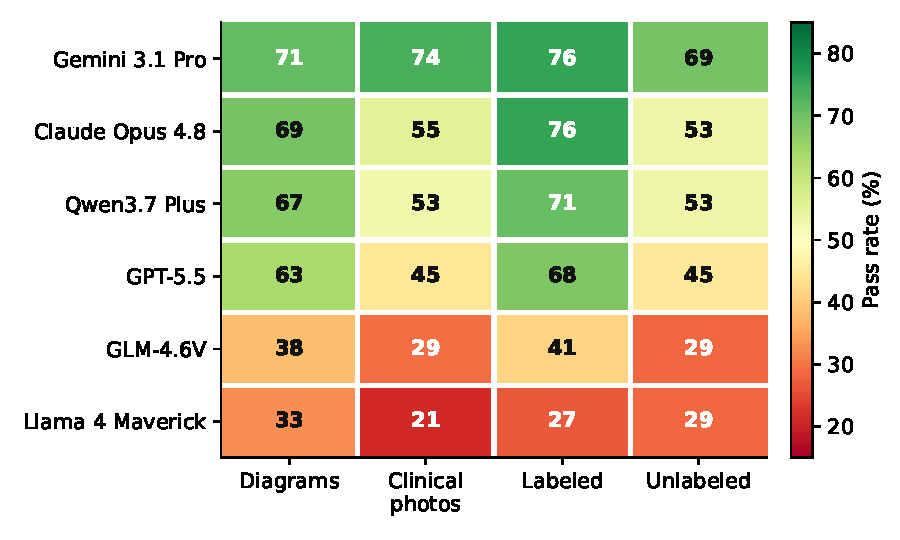
\includegraphics[width=0.78\linewidth]{figures/task_split.pdf}
\caption{Pass rate by model and task split. Diagrams and labeled images are read more reliably than unlabeled clinical photographs across the field.}
\label{fig:split}
\end{figure}

\subsection{Paired model comparisons}

Because every model is scored on the same 90 images, model comparisons are paired by item, and McNemar tests are more appropriate than comparing independent Wilson intervals. Across the 15 model pairs (McNemar exact test, Holm-corrected; item-level bootstrap intervals from 10{,}000 resamples), 9 of 15 differences are significant at $p<0.05$ (Figure~\ref{fig:pairwise}). The three leading models are statistically indistinguishable: \model{Gemini 3.1 Pro} versus \model{Claude Opus 4.8} ($\Delta=+9$ points, $p=0.93$), \model{Gemini 3.1 Pro} versus \model{Qwen3.7 Plus} ($+11$, $p=0.32$), and \model{Claude Opus 4.8} versus \model{Qwen3.7 Plus} ($+2$, $p=1.0$). \model{Gemini 3.1 Pro} is significantly above \model{GPT-5.5} ($+17$, $p=0.04$), the leading cluster is significantly above \model{GLM-4.6V} and \model{Llama 4 Maverick}, and those two are themselves indistinguishable ($p=1.0$). This paired analysis formally supports the headline reading: a leading cluster rather than a resolved ranking, separated from a lower-performing tail.

\begin{figure}[t]
\centering
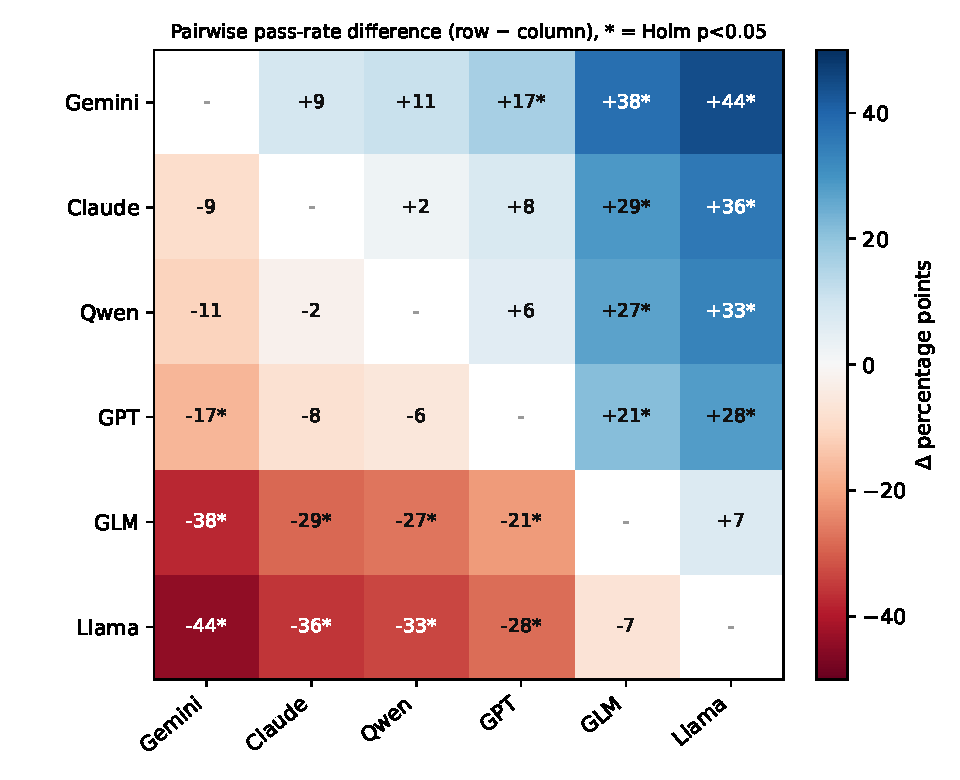
\includegraphics[width=0.82\linewidth]{figures/pairwise.pdf}
\caption{Pairwise pass-rate differences (row minus column, percentage points); an asterisk marks a Holm-corrected McNemar $p<0.05$.}
\label{fig:pairwise}
\end{figure}

A mixed-effects logistic regression with a random intercept per image, and fixed effects for model, modality, labeled status, and weak-item flag, clarifies the task split. The strongest controllable factor is text labeling: labeled images have 2.2 times the odds of a passing description (95\% credible interval [1.6, 3.1]) relative to unlabeled images. Once labeling and item difficulty are accounted for, the diagram-versus-clinical-photograph difference is small and its 95\% credible interval crosses 1 (odds ratio 0.84, [0.59, 1.19]), so the apparent diagram advantage in Table~\ref{tab:results} is largely explained by diagrams more often carrying readable labels. Weak or ambiguous items are much harder, as expected (odds ratio 0.12, [0.05, 0.25]). Finally, we did not detect evidence that longer rubrics made items harder: the pooled pass rate is flat to non-monotonic from 2 to 6 required points, and an item-clustered logistic regression shows no significant effect of the number of \emph{must identify} points (odds ratio 1.23 per point, [0.82, 1.83], $p=0.32$). With only 3 items at 2 required points and 2 at 6, however, this null rests on small numbers at the extremes.

\subsection{Judge agreement}

The two judges returned the same pass/fail verdict on 82\% of descriptions, with Cohen's $\kappa=0.65$ (Table~\ref{tab:judges}). The primary judge (\model{Claude Opus 4.8}) was more lenient than the secondary judge (\model{GPT-5.5}) for every model. \model{Claude Opus 4.8} had the \emph{smallest} primary-versus-secondary gap (+7 points), not the largest, which is not what a simple self-preference effect would predict. This delta is only suggestive, however: it conflates the secondary judge's overall strictness with any self-preference, and because the reported leaderboard uses the more lenient primary judge, the design cannot cleanly separate leniency from self-preference. The defensible reading is that absolute pass rates are strongly judge-dependent and should not be taken on faith. Under the secondary judge, \model{Claude Opus 4.8} (56\%) scores above \model{Gemini 3.1 Pro} (50\%), so even the top of the order is not stable across judges; this reinforces that the leading cluster should not be read as a resolved ranking.

\begin{table}[t]
\centering
\caption{Judge agreement. Pass rate assigned by the primary (\model{Claude Opus 4.8}) and secondary (\model{GPT-5.5}) judges, and their difference. Overall verdict agreement 82\%, Cohen's $\kappa=0.65$.}
\label{tab:judges}
\begin{tabular}{lrrr}
\toprule
Model & Primary judge & Secondary judge & $\Delta$ \\
\midrule
Gemini 3.1 Pro & 72\% & 50\% & +22 \\
Claude Opus 4.8 & 63\% & 56\% & +7 \\
Qwen3.7 Plus & 61\% & 47\% & +14 \\
GPT-5.5 & 56\% & 36\% & +20 \\
GLM-4.6V & 34\% & 16\% & +18 \\
Llama 4 Maverick & 28\% & 11\% & +17 \\
\bottomrule
\end{tabular}
\end{table}

\subsection{Transformed control}

The transformed control is a single item, a flipped and cropped copy of one public anatomy diagram whose original is passed by all six models, so it is a weak format-robustness sanity check rather than a memorization measurement. Under the primary judge, every model returned the same pass verdict on the control as on the original; under the secondary judge, the two weakest models (\model{GLM-4.6V} and \model{Llama 4 Maverick}) flipped from pass to fail on the transformed copy. The check is consistent with image reading rather than exact-image recognition of the public files, but a single ceiling-level item cannot establish that on its own.

\subsection{Contamination and held-out evaluation}

The public images are openly licensed and crawlable, so training-data exposure is a genuine threat to validity \cite{contamination2025survey}. Two guards address it at the level a public dataset allows: the leakage guard at input removes the caption and any web access, and the transformed-control check found no exact-image recognition effect. Neither substitutes for a definitive contamination test, which requires a held-out set of non-public images matched in content and difficulty to the public set; constructing and running that set is the central item of future work.

\section{Discussion}

Contemporary vision language models can read many dental diagrams and labeled images, but this benchmark shows why specialty-specific, open-ended evaluation remains necessary. The leading systems cluster tightly with overlapping intervals, so a ranking from 90 images would be overconfident; the defensible conclusion is that a leading cluster (\model{Gemini 3.1 Pro}, \model{Claude Opus 4.8}, \model{Qwen3.7 Plus}) performed substantially better than the lower-performing tail, and that the stable signal is task dependence, not the rank order: readable labels are the strongest controllable factor and unlabeled clinical images are the hardest clinically relevant condition. Strength on text-based clinical question answering need not predict vision-reading rank, which cautions against transferring text leaderboards to vision tasks. This benchmark is complementary to larger dental image resources such as MetaDent \cite{li2026metadent}: where MetaDent emphasizes scale, semi-structured annotation, and visual question answering or classification over mostly intraoral photographs, this work emphasizes small-scale, caption-free, open-ended description across diagrams and clinical photographs, graded by explicit clinician pass/fail rubrics and two image-grounded judges with per-row auditability.

The open-ended, rubric-graded design exposes failures that closed question-answering can hide. A description can be fluent and confident yet fail because it omits a required finding or commits a prohibited error, and the unlabeled clinical-photograph column is where that happens most. For a clinician or educator deciding which model to trust with an unlabeled intraoral photograph, the right summary is not a single winner but a task-conditioned expectation: reading diagrams and labeled images is markedly easier (the best models reach about 70\% on diagrams) than reading an unlabeled real mouth, though neither is solved.

The method is intentionally small and preliminary. The benchmark uses a single trial, an LLM-judge layer whose absolute scores are judge-dependent, and ground truth from two dentists rather than a large consensus panel. The secondary-judge pass and the released judge-disagreement worklist quantify the judge problem rather than solve it; prespecified human adjudication of the disagreement set is the natural next step.

\section{Limitations}

First, the benchmark contains 90 images; the Wilson intervals are correspondingly wide and small differences should be treated as noise. Second, the run used a single trial at temperature 0; run-to-run stability was not measured. Third, ground truth was authored by one periodontist and confirmed by one independent dentist, which is stronger than single-author ground truth but is not a multi-expert consensus panel, and the independent reviewer reported agreement rather than adjudicating judge disagreements. Fourth, all pass/fail verdicts rely on model judges that, while in substantial agreement by the Landis--Koch scale ($\kappa=0.65$), are themselves evaluated models, and the two judges differ enough that absolute pass rates are judge-dependent. Fifth, contamination cannot be fully excluded for openly licensed images, and a content-matched held-out evaluation is left to future work. Sixth, results reflect model versions and OpenRouter routing on June 15--16, 2026 (the main run on June 15, with 7 transient-error rows re-run on June 16), which may drift. Finally, the benchmark scores text descriptions of dental images; it does not validate clinical deployment, diagnosis, or patient outcomes, and radiographic interpretation is out of scope.

\section{Data and Code Availability}

The images, clinician rubrics, per-row results, both judges' verdicts, the run manifest, the analysis and figure scripts, the validation record, and an interactive report are available at:
\begin{center}
\url{https://github.com/Tuminha/dental-vision-benchmark}
\end{center}
The data, code, manuscript source, and figures are released at the following versions:
\begin{center}
\begin{tabular}{ll}
\toprule
Component & Identifier \\
\midrule
Released data snapshot & git commit \texttt{9fa7576} \\
Software release (latest) & \texttt{v1.0.1} \\
Concept DOI (all versions) & Zenodo \texttt{10.5281/zenodo.20722369} \\
This-version DOI & Zenodo \texttt{10.5281/zenodo.20722424} \\
\bottomrule
\end{tabular}
\end{center}
Images are openly licensed and keep their own licenses; the benchmark code is MIT. An interactive report is at \url{https://tuminha.github.io/dental-vision-benchmark/}.

\section{Ethics Statement}

No new human-subject data were collected by the authors. The study used publicly available, openly licensed images and non-patient model outputs; per-image source, license, and attribution are provided. The need for ethics approval was considered not applicable under this study design, and the study did not use patient records or protected health information. The results should not be interpreted as validating any model for autonomous diagnosis, treatment planning, or patient-specific clinical decision-making.

\section{Funding}

This work received no external funding.

\section{Competing Interests}

F.T.B. is the founder of Periospot and Executive Director of the Foundation for Oral Rehabilitation; neither organization had a role in the study design, data collection, analysis, or the decision to publish. The authors declare no other competing interests.

\section{Author Contributions}

F.T.B. designed the benchmark, curated and authored the dataset and rubrics, implemented the evaluation harness, ran the analyses, and drafted the manuscript. D.R.C. performed independent clinical validation of the ground truth and contributed clinical and scientific review.

\section{Acknowledgments}

The authors acknowledge the Foundation for Oral Rehabilitation and Periospot for support during preparation of this benchmark and manuscript.

\section{Declaration of Generative AI and AI-Assisted Technologies}

During preparation of this work, the authors used GPT-5.5 Pro and Claude Code to assist with manuscript critique, wording refinement, code review, statistical implementation, and consistency checking. The authors reviewed, verified, edited, and take full responsibility for all manuscript content, analyses, code, references, and conclusions. No AI system is listed as an author.

\begin{thebibliography}{99}
\raggedright

\bibitem{hu2024omnimedvqa}
Y.~Hu, T.~Li, Q.~Lu, W.~Shao, J.~He, Y.~Qiao, and P.~Luo.
\newblock OmniMedVQA: A new large-scale comprehensive evaluation benchmark for medical LVLM.
\newblock In \emph{CVPR}, 2024. arXiv:2402.09181.

\bibitem{chen2024gmaimmbench}
P.~Chen, J.~Ye, G.~Wang, Y.~Li, Z.~Deng, W.~Li, T.~Li, et~al.
\newblock GMAI-MMBench: A comprehensive multimodal evaluation benchmark towards general medical AI.
\newblock In \emph{NeurIPS Datasets and Benchmarks}, 2024. \url{https://openreview.net/forum?id=K6b8LCXBeQ}.

\bibitem{wang2026oralmllm}
R.~Wang, S.~Zhou, J.~Wang, W.~Xie, and X.~Che.
\newblock OralMLLM-Bench: Evaluating cognitive capabilities of multimodal large language models in dental practice.
\newblock arXiv:2605.01333, 2026.

\bibitem{li2026metadent}
M.-X. Li, W.-H. Deng, Z.-X. Wu, C.-X. Jin, J.-M. Wu, Y.~Han, J.~K.~H. Tsoi, G.-S. Xia, and C.~Huang.
\newblock MetaDent: Labeling clinical images for vision-language models in dentistry.
\newblock \emph{Journal of Dental Research}, 2026. doi:10.1177/00220345261424242.

\bibitem{lv2026orodental}
H.~Lv, I.~Haq, J.~Du, J.~Ma, B.~Zhu, X.~Dang, C.~Liang, R.~Du, Y.~Zhang, and M.~Saqib.
\newblock A benchmark multimodal oro-dental dataset for large vision-language models.
\newblock \emph{Scientific Data}, 2026. doi:10.1038/s41597-026-07342-9. arXiv:2511.04948.

\bibitem{zhu2025dentalbench}
H.~Zhu, Y.~Xu, Y.~Li, Z.~Meng, and Z.~Liu.
\newblock DentalBench: Benchmarking and advancing LLMs capability for bilingual dentistry understanding.
\newblock arXiv:2508.20416, 2025.

\bibitem{nguyen2025omf}
V.~A. Nguyen, T.~Q.~T. Vuong, and V.~H. Nguyen.
\newblock Benchmarking large-language-model vision capabilities in oral and maxillofacial anatomy: A cross-sectional study.
\newblock \emph{PLoS One}, 2025. PMC12561936.

\bibitem{zheng2023judge}
L.~Zheng, W.-L. Chiang, Y.~Sheng, S.~Zhuang, Z.~Wu, Y.~Zhuang, Z.~Lin, Z.~Li, D.~Li, E.~P. Xing, et~al.
\newblock Judging LLM-as-a-judge with MT-Bench and Chatbot Arena.
\newblock In \emph{NeurIPS Datasets and Benchmarks}, 2023. arXiv:2306.05685.

\bibitem{arora2025healthbench}
R.~K. Arora, J.~Wei, R.~Soskin Hicks, P.~Bowman, J.~Quinonero-Candela, F.~Tsimpourlas, M.~Sharman, M.~Shah, A.~Vallone, A.~Beutel, J.~Heidecke, and K.~Singhal.
\newblock HealthBench: Evaluating large language models towards improved human health.
\newblock arXiv:2505.08775, 2025.

\bibitem{panickssery2024selfrecognition}
A.~Panickssery, S.~R. Bowman, and S.~Feng.
\newblock LLM evaluators recognize and favor their own generations.
\newblock arXiv:2404.13076, 2024.

\bibitem{wataoka2024selfpreference}
K.~Wataoka, T.~Takahashi, and R.~Ri.
\newblock Self-preference bias in LLM-as-a-judge.
\newblock arXiv:2410.21819, 2024.

\bibitem{contamination2025survey}
S.~Chen, Y.~Chen, Z.~Li, Y.~Jiang, Z.~Wan, Y.~He, D.~Ran, T.~Gu, H.~Li, T.~Xie, and B.~Ray.
\newblock Recent advances in large language model benchmarks against data contamination: From static to dynamic evaluation.
\newblock arXiv:2502.17521, 2025.

\end{thebibliography}

\end{document}
